% This LaTeX was auto-generated from MATLAB code.
% To make changes, update the MATLAB code and export to LaTeX again.

\documentclass{article}

\usepackage[utf8]{inputenc}
\usepackage[T1]{fontenc}
\usepackage{lmodern}
\usepackage{graphicx}
\usepackage{color}
\usepackage{hyperref}
\usepackage{amsmath}
\usepackage{amsfonts}
\usepackage{epstopdf}
\usepackage[table]{xcolor}
\usepackage{matlab}
\usepackage{geometry}

\sloppy
\epstopdfsetup{outdir=./}
\graphicspath{ {./main_images/} }

\geometry{left=1.0in,right=1.0in,top=1.0in,bottom=1.0in}

\begin{document}

\matlabtitle{Homework 1 Report}

\begin{matlabcode}
addpath('/Applications/Dynare/4.6.2/matlab'); % add dynare path
\end{matlabcode}
We use Dynare 4.6.2 for this homework. Dynare 4.6 has changed the usage of some functions, for example, \textit{stoch\_simul}, and thus the code may not work for a lower version.

\section*{Exercise 4.10} 


Before starting Q1, we first replicate the right panel of table 4.2 in the textbook to ensure our model, variable definitions, and solution method are consistent with the textbook.

\begin{matlabcode}
dynare Q410.mod; 
print_table()    % exactly replicate table 4.2 using textbook calibration
\end{matlabcode}
\begin{matlaboutput}
Results of table 4.2:

Variable  sig_x       rho1       rho2
   y       3.08       0.62       1.00
   c       2.71       0.78       0.84
   i       9.04       0.07       0.67
   h       2.12       0.62       1.00
tb_y       1.78       0.51      -0.04
ca_y       1.45       0.32       0.05
\end{matlaboutput}

\subsection*{Q1. Calibrate the EDEIR Model for Canada 1960-2011}

\begin{matlabcode}
%{
NOTE:
    1. moments to match: [std(y),autocor(y),std(i),std(tb/y)]
    2. target moment values: [3.71%, 0.86, 10.31%, 1.72%]
    3. pars to calibrate: rho, eta, phi, psi_1
    4. method: min distance
    5. solver: fminunc/BFGS Quasi-Newton
    6. init guess: param = [0.42 0.0129 0.028 0.000742]
%}

param_init = [0.42 0.0129 0.028 0.000742];
param_est  = fminunc(@(x)m_dist(x), param_init);

fprintf('Estimation results:\n');
fprintf('\n');
fprintf('rho   = %.6f\n', param_est(1));
fprintf('eta   = %.6f\n', param_est(2));
fprintf('phi   = %.6f\n', param_est(3));
fprintf('psi_1 = %.6f\n', param_est(4));
\end{matlabcode}

\begin{matlaboutput}
Estimation results:

rho   = 0.621901
eta   = 0.010536
phi   = 0.018179
psi_1 = 0.026189
\end{matlaboutput}

Thus, we get a higher $\rho$ and $\psi_1$ but a lower $\eta$ and $\phi$.



\subsection*{Q2. Compute the Theoretical Second Moments}

We employ the estimated parameters to re-solve the model. Dynare automatically reports the theoretical moments for 1st order solutions.
\begin{matlabcode}
% Q2 Compute theoretical second moments

set_param_value('rho',  param_est(1)); 
set_param_value('eta',  param_est(2));
set_param_value('phi',  param_est(3)); 
set_param_value('psi_1',param_est(4));

[info,oo_,options_,M_] = stoch_simul(M_,options_,oo_,var_list_);

print_table()
\end{matlabcode}

\begin{matlaboutput}
Results of table 4.2:

Variable  sig_x       rho1       rho2
   y       3.71       0.84       1.00
   c       3.18       0.89       0.98
   i      10.31       0.16       0.64
   h       2.55       0.84       1.00
tb_y       1.73       0.04      -0.12
ca_y       1.66       0.04      -0.07
\end{matlaboutput}

\subsection*{Q3. Comment}

\begin{itemize}
    \item The model does a good job in generating the observed standard deviation of output $y$, investment $i$, and trade-balance-to-output ratio $\frac{tb}{y}$.\\
    But this is not surprising because that is how we calibrate the model using the SMM. 
    
    \item The model does a poor job in explaining the autocorrelation of $i$ and $\frac{tb}{y}$, which are much less correlated than in the data.

    \item The model also does a poor job in explaining the correlation between $y$ and $\frac{tb}{y}$. Its sign is the opposite of the one in the data.
\end{itemize}

\subsection*{Q4. TFP Shock and Output Volatility}

\begin{matlabcode}
% Q4 compute std(ln A)
sd_list  = sqrt(diag(oo_.var));
sd_A     = sd_list(strcmp('A',M_.endo_names))*100;
sd_y     = sd_list(strcmp('y',M_.endo_names))*100;
sd_A_old = 100*sqrt(0.0129^2/(1-0.42^2));

fprintf('Unconditional SD(ln(A)) = %.4f\n', sd_A);
fprintf('Old value:                %.4f\n', sd_A_old);

fprintf('Unconditional SD(y)     = %.4f\n', sd_y);
fprintf('Old value:                %.4f\n', 3.08);
\end{matlabcode}

\begin{matlaboutput}
Unconditional SD(ln(A)) = 1.3455
Old value:                1.4214
Unconditional SD(y)     = 3.7130
Old value:                3.0800
\end{matlaboutput}

From the results above we can see that 
\begin{itemize}
    \item the volatility of TFP shock has actually \textbf{decreased}; 
    \item On the other hand, the volatility of output has \textbf{increased}. 
\end{itemize}
This means the business cycle relies less on the TFP shock. However, its internal amplification and propagation mechanisms have become stronger than in the past. The latter effect outweighs the previous effect, and as a result, the overall output volatility still increases.


\newpage

\section*{Exercise 6.5}
\subsection*{Q1. The EDEIR Model}
\begin{matlabcode}
%---------------- EDEIR ------------------
% replicate column 4 of table 4.4
% make sure the results generated by the new model is consistent with the old results

dynare EDEIR
\end{matlabcode}
\begin{matlaboutput}
THEORETICAL MOMENTS
VARIABLE         MEAN  STD. DEV.   VARIANCE
y              0.3964     0.0308     0.0010
c              0.1106     0.0271     0.0007
i             -1.0795     0.0904     0.0082
h              0.0074     0.0212     0.0004
tb_y           0.0200     0.0178     0.0003
ca_y           0.0000     0.0145     0.0002

MATRIX OF CORRELATIONS
Variables         y       c       i       h    tb_y    ca_y
y            1.0000  0.8440  0.6688  1.0000 -0.0435  0.0503
c            0.8440  1.0000  0.5177  0.8440 -0.3114  0.0654
i            0.6688  0.5177  1.0000  0.6688 -0.6178 -0.7068
h            1.0000  0.8440  0.6688  1.0000 -0.0435  0.0503
tb_y        -0.0435 -0.3114 -0.6178 -0.0435  1.0000  0.8318
ca_y         0.0503  0.0654 -0.7068  0.0503  0.8318  1.0000

COEFFICIENTS OF AUTOCORRELATION
Order          1       2       3       4       5
y         0.6170  0.3603  0.2066  0.1201  0.0733
c         0.7822  0.6367  0.5493  0.4996  0.4721
i         0.0686 -0.1379 -0.1363 -0.0935 -0.0553
h         0.6170  0.3603  0.2066  0.1201  0.0733
tb_y      0.5086  0.3484  0.3028  0.2938  0.2945
ca_y      0.3220  0.0875  0.0130 -0.0067 -0.0096
Total computing time : 0h00m01s
\end{matlaboutput}
\begin{matlabcode}
% turn off productivity shock and turn on interest rate shock
set_param_value('eta', 0);
set_param_value('sigma_mu', 0.012);
% re-run the model
options_.irf = 20;
[info,oo_,options_,M_]=stoch_simul(M_,options_,oo_,var_list_);
\end{matlabcode}
\begin{matlaboutput}
THEORETICAL MOMENTS
VARIABLE         MEAN  STD. DEV.   VARIANCE
y              0.3964     0.1560     0.0243
c              0.1106     0.1092     0.0119
i             -1.0795     0.9933     0.9866
h              0.0074     0.1072     0.0115
tb_y           0.0200     0.2417     0.0584
ca_y           0.0000     0.2377     0.0565

MATRIX OF CORRELATIONS
Variables         y       c       i       h    tb_y    ca_y
y            1.0000  0.9932  0.0635  1.0000  0.2357  0.1869
c            0.9932  1.0000  0.1636  0.9932  0.1351  0.0867
i            0.0635  0.1636  1.0000  0.0635 -0.9547 -0.9684
h            1.0000  0.9932  0.0635  1.0000  0.2357  0.1869
tb_y         0.2357  0.1351 -0.9547  0.2357  1.0000  0.9985
ca_y         0.1869  0.0867 -0.9684  0.1869  0.9985  1.0000

COEFFICIENTS OF AUTOCORRELATION
Order          1       2       3       4       5
y         0.9243  0.7986  0.6670  0.5468  0.4435
c         0.9411  0.8189  0.6852  0.5610  0.4535
i         0.3708  0.0914 -0.0249 -0.0668 -0.0759
h         0.9243  0.7986  0.6670  0.5468  0.4435
tb_y      0.3330  0.0432 -0.0720 -0.1085 -0.1111
ca_y      0.3197  0.0368 -0.0752 -0.1102 -0.1120
\end{matlaboutput}
\begin{center}
\includegraphics[width=.75\linewidth]{figure_0.png}
\end{center}





\subsection*{Q2. The IDF Model}

\begin{matlabcode}
%---------------- IDF --------------------
% replicate column 1 of table 4.4
% make sure the results generated by the new model is consistent with the old results

dynare IDF
\end{matlabcode}
\begin{matlaboutput}
THEORETICAL MOMENTS
VARIABLE         MEAN  STD. DEV.   VARIANCE
y              0.3964     0.0307     0.0009
c              0.1106     0.0235     0.0006
i             -1.0795     0.0910     0.0083
h              0.0074     0.0211     0.0004
tb_y           0.0200     0.0155     0.0002
ca_y           0.0000     0.0146     0.0002

MATRIX OF CORRELATIONS
Variables         y       c       i       h    tb_y    ca_y
y            1.0000  0.9376  0.6581  1.0000 -0.0122  0.0263
c            0.9376  1.0000  0.5581  0.9376 -0.0701  0.0623
i            0.6581  0.5581  1.0000  0.6581 -0.7025 -0.7301
h            1.0000  0.9376  0.6581  1.0000 -0.0122  0.0263
tb_y        -0.0122 -0.0701 -0.7025 -0.0122  1.0000  0.9609
ca_y         0.0263  0.0623 -0.7301  0.0263  0.9609  1.0000

COEFFICIENTS OF AUTOCORRELATION
Order          1       2       3       4       5
y         0.6122  0.3505  0.1925  0.1029  0.0539
c         0.6988  0.4959  0.3725  0.3010  0.2604
i         0.0700 -0.1405 -0.1415 -0.0995 -0.0612
h         0.6122  0.3505  0.1925  0.1029  0.0539
tb_y      0.3268  0.1113  0.0531  0.0440  0.0473
ca_y      0.3022  0.0657 -0.0061 -0.0228 -0.0232
Total computing time : 0h00m01s
Note: warning(s) encountered in MATLAB/Octave code
\end{matlaboutput}
\begin{matlabcode}

% turn off productivity shock and turn on interest rate shock
set_param_value('sigma_tfp', 0);
set_param_value('sigma_mu',  0.012);

% re-run the model
options_.irf = 20; 
[info,oo_,options_,M_]=stoch_simul(M_,options_,oo_,var_list_);
\end{matlabcode}
\begin{matlaboutput}
THEORETICAL MOMENTS
VARIABLE         MEAN  STD. DEV.   VARIANCE
y              0.3964     0.1622     0.0263
c              0.1106     0.1162     0.0135
i             -1.0795     1.0224     1.0454
h              0.0074     0.1115     0.0124
tb_y           0.0200     0.2513     0.0632
ca_y           0.0000     0.2470     0.0610

MATRIX OF CORRELATIONS
Variables         y       c       i       h    tb_y    ca_y
y            1.0000  0.9884  0.0684  1.0000  0.2254  0.1724
c            0.9884  1.0000  0.2005  0.9884  0.0912  0.0388
i            0.0684  0.2005  1.0000  0.0684 -0.9562 -0.9709
h            1.0000  0.9884  0.0684  1.0000  0.2254  0.1724
tb_y         0.2254  0.0912 -0.9562  0.2254  1.0000  0.9983
ca_y         0.1724  0.0388 -0.9709  0.1724  0.9983  1.0000

COEFFICIENTS OF AUTOCORRELATION
Order          1       2       3       4       5
y         0.9259  0.8018  0.6712  0.5513  0.4481
c         0.9436  0.8205  0.6843  0.5570  0.4464
i         0.3781  0.0976 -0.0214 -0.0654 -0.0758
h         0.9259  0.8018  0.6712  0.5513  0.4481
tb_y      0.3422  0.0515 -0.0666 -0.1056 -0.1099
ca_y      0.3282  0.0438 -0.0712 -0.1086 -0.1119
\end{matlaboutput}


\begin{center}
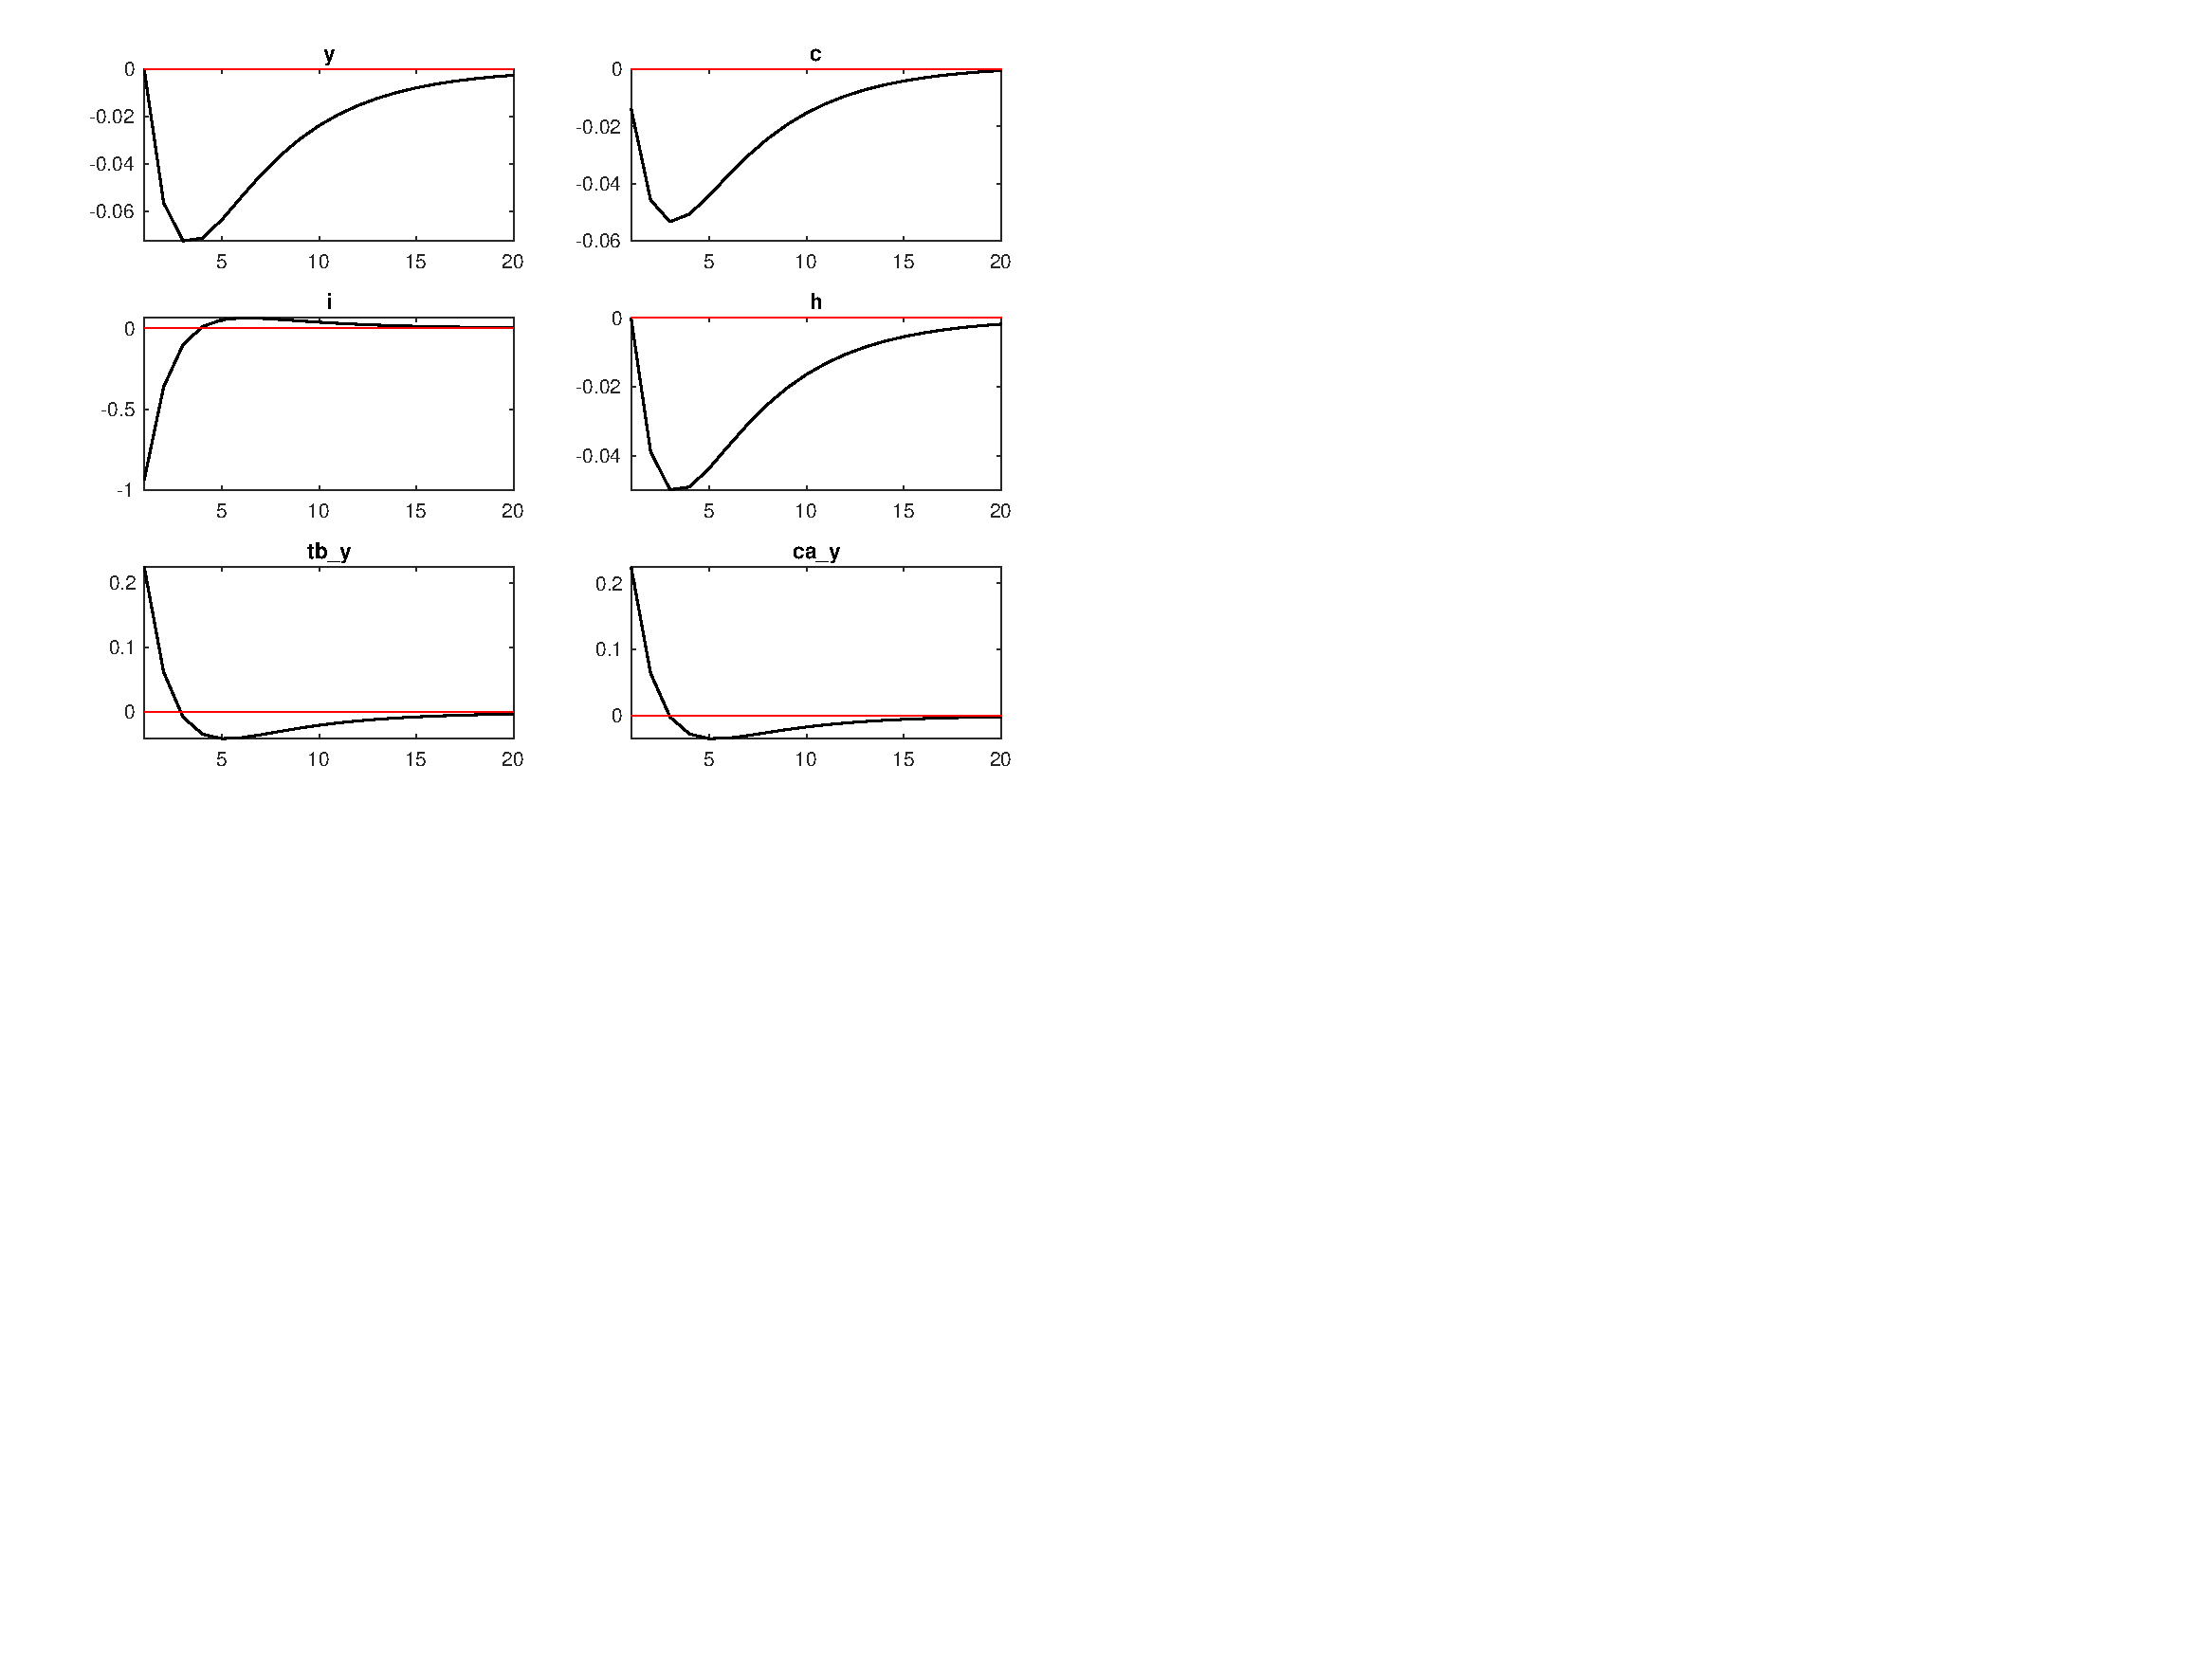
\includegraphics[width=.75\linewidth]{figure_1.pdf}
\end{center}

\end{document}
